\title{60-371\\Artificial Intelligence\\Iterated Prisoner's Dilemma}
\author{
		Quinn Perfetto \\
        William Roeder \\
        David Valleau
}
\date{\today}

\documentclass[12pt]{article}

\usepackage{ amssymb }
\usepackage{longtable}
\usepackage[T1]{fontenc}
\usepackage{tocloft}
\usepackage{hyperref}
\usepackage[none]{hyphenat}
\usepackage[]{algorithm2e}
\usepackage{graphicx}
\hypersetup{
    colorlinks=true,
    linkcolor=black,
    urlcolor=blue
}
\renewcommand\cftsecleader{\cftdotfill{\cftdotsep}}
\setlength\parindent{0pt}

\SetKwInput{KwInput}{Input}
\SetKwInput{KwOutput}{Output}

\begin{document}
\maketitle

\pagebreak
\tableofcontents
\pagebreak

\section{Abstract}

This paper explores two Artificial Intelligence algorithms used
to create optimal strategies to compete in the Iterated Prisoner's Dilemma. The
study begins by examining the use of a genetic algorithm to breed the perfect
prisoner. This is achieved by contrasting the performance of a variety of different configurations and fitness functions.  The genetic algorithm was able to
consistently breed well performing prisoners.
A hill climbing approach was then taken, which proved to be ineffective at producing a competitive strategy given the
lack of a natural successor function and no clear end goal.  The traits
of a strong genome are explored and finally, the performance of the two methods are contrasted.

\pagebreak

\section{Introduction}
The Iterated Prisoner's Dilemma is a classic example of game theory which demonstrates
that two agents acting for their own self interest may not result in an
optimal outcome for either agent.  The prisoner's
dilemma is as follows: \\ \\
Two individuals (herein Bob and Alice) have been arrested and placed in solitary
confinement, meaning they may not communicate with one another.  Each of them hope
to spend the least amount of time in prison. The prosecutor approaches them
and offers them the following deal:
\begin{itemize}
    \item If Bob and Alice betray (herein defect) each other, they will
        both serve 2 years in prison
    \item If Bob defects but Alice remains silent (herein cooperate), Bob
        will be set free and Alice will spend 3 years in prison (and vice versa)
    \item If Bob and Alice both cooperate they will each spend 1 year in prison
        on a lesser charge \\
\end{itemize}

The iterated version of the prisoner's dilemma is simply a sequence of rounds of
the above mentioned game.  A player's resulting score is the summation of their score in
each round. \\

It is implied that Bob and Alice will have no interactions with each other after
their decisions. Therefore, they cannot punish/reward their accomplice. If Bob and Alice are
both rational and self centered individuals then they will both choose to defect, 
as defecting yields the highest probability of a favourable outcome.
It is interesting to note
that if the prisoners act non-rationally and choose to cooperate, a "riskier" option, they will spend one third of the time in prison when compared
to the rational option. \\

Taking after J. Golbeck
\footnote{\href{http://cgis.cs.umd.edu/~golbeck/downloads/JGolbeck\_prison.pdf}
{Evolving Strategies for the Prisoner's Dilemma}}
the payoff matrix for this study (seen below) has been
inverted such that a higher score implies a lesser sentence. \\

\begin{center}
    \begin{tabular}{l | c | c}
         & Cooperate & Defect \\
        \hline
        Cooperate & (3,3) & (5, 0)\\
        \hline
        Defect & (0, 5) & (1,1) \\ \\
    \end{tabular}
\end{center}

Iterated prisoner's dilemma strategies have been widely studied, and many have
concluded that Tit-for-Tat (herein TFT) produces the best average performance.
TFT is exceedingly simple: Cooperate on the first turn, mirror the opponents
last move thereafter.  TFT is effective because it capitalizes on mutual
cooperation, but is also able to defend itself against rogue defectors.  These
two qualities are extremely important and were kept in mind when designing the
algorithms explained in this paper.
\section{Genetic Algorithm}

The genetic algorithm in this paper has a structure equivalent to: \\

\begin{algorithm}[H]
 \KwResult{An evolved genetic prisoner}
 population = [] \;
 \For{$i\leftarrow 1$ \KwTo $popSize$}{
    Push(population, RandomPrisoner())\;
  }
 \For{$g\leftarrow 1$ \KwTo $generation$}{
  evaluation = EvaluateFitness(population)\;
  selection  = WeightedRandomSample(evaluation)\;
  cross      = CrossOver(selection)\;
  population = Mutate(cross);
 }
 \KwRet{MaxFitness(population)}
\end{algorithm}

\subsection{Representation}
Each genetic prisoner's strategy is represented as a vector of size
$4^n$ where $n$ is the number of moves the prisoner keeps in memory.  This vector
is thought of as the prisoner's "genome".
The prisoner's move is then calculated by encoding the last $n$ rounds of the game
into an integer and indexing the strategy vector at that point. \\

For example if Bob has
a memory size of one, a possible strategy vector would be
$S_B = [C, C, D, C]$.  If in the previous round Bob cooperated and Alice defected,
the corresponding history string would be represented as $DC$.
The history string is then
marshalled into a base two integer by changing Defections to 0's and Cooperations
to 1's, yielding $01$.  The strategy vector is then indexed at the base
10 representation giving ${S_B}_1 = C$, thus Bob will Cooperate. \\

All examples below use a memory size of three as it was observed to yield the
highest average score seen in \hyperref[fig1]{Figure 1}.

\begin{figure}[h]
    \centering
    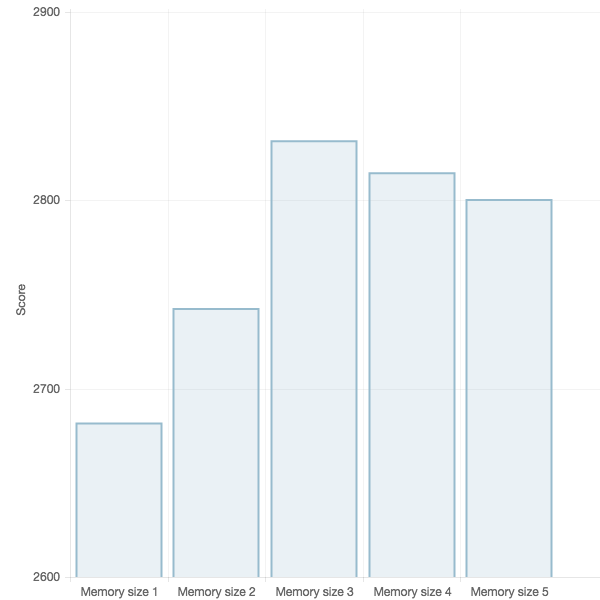
\includegraphics[scale=0.6]{figures/memsize-vs-score.png}
    \label{fig1}
    \caption{Graph of memory size vs average score over 100 games}
\end{figure}

\subsection{Initial Population}
The initial population was a pool of prisoners having completely randomized
strategy vectors.  The population size was variable, and the effects of varying
sizes are explained in \textit{\hyperref[vpg]{section 3.7}}

\subsection{Fitness Function}

Three different fitness functions were used to evaluate a prisoner's performance.
A description of each, as well as their performance comparisons, follow.

\subsubsection{Score Against Diverse Opponents}
The prisoner being evaluated would play 100 rounds against a selection of nine
strategies which were thought to be a uniform representation of all possible
strategies.  Total score was calculated and used as a performance grade.
The nine strategies were:
\begin{enumerate}
    \item All C - Always cooperate
    \item All D - Always defect
    \item Tit for Tat - Cooperate first move, mirror opponents last move thereafter
    \item Suspicious Tit for Tat - Defect first move, mirror opponents last move
        thereafter
    \item Tit for 2 Tat - Cooperate first two moves, only cooperate if the
        opponent did not defect twice in a row thereafter
    \item Suspicious Tit for 2 Tat - Defect first two moves, only cooperate if the
        opponent did not defect twice in a row thereafter
    \item Grudger - Cooperate until the opponent defects, then defect without mercy
    \item Sucker - Defect until the opponent cooperates, then cooperate foolishly
    \item Hesitant - Only cooperate if the opponent has cooperated twice in a row
\end{enumerate}

From a shallow point of view this method of evaluating fitness was mostly
successful.  After some contemplation it was decided that the
nine strategies used were slightly biased towards those which tended to cooperate.
This left some of the prisoners produced vulnerable to rogue defectors,
and thus sub-optimal.

\subsubsection{Hamming Distance From TFT Genome}
The prisoner would be evaluated based on the hamming distance
\footnote
{\href{https://en.wikipedia.org/wiki/Hamming distance}{Hamming Distance}}
between its current strategy vector and the strategy vector representing
the TFT genome.  This obviously had a tendency to produce prisoners which
acted increasingly similar to TFT.  Although the performance of said bots
was sound, this method did not produce any extraordinary or new strategies.

\subsubsection{Score Against TFT}
\label{tft}

The prisoner would be evaluated based on its score after 100 rounds against
TFT.  Since TFT is widely accepted as one of the best overall strategies, it was
decided that performance against it would be a suitable benchmark.
This method seemed to produce the best results with the least
amount of computation time.  The prisoners behaved somewhat similarly
to TFT but contained some genome sections which differed considerably.  The result was a prisoner which \textit{mostly} contained the desired qualities from TFT
but also included some routines which gave it an advantage in certain situations.


\subsubsection{Fitness Function Comparison}

\begin{figure}[h]
    \label{fig2}
    \centering
    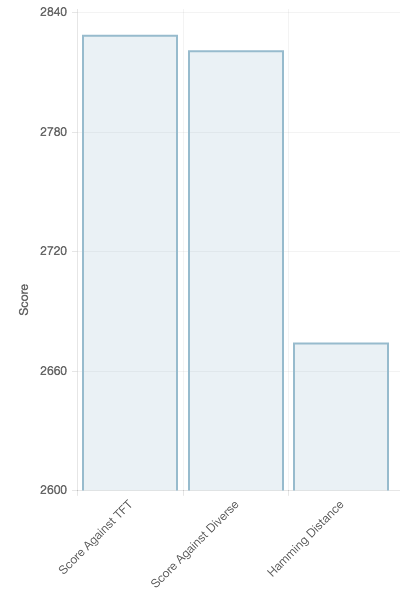
\includegraphics[scale=0.5]{figures/fit_score.png}
    \label{fig1}
    \caption{Graph of fitness function vs average score over 100 games}
\end{figure}

As evidenced by \hyperref[fig2]{Figure 2} Score against TFT and Score Against Diverse
produced very similar average scores (within 10 points).  The main difference
between the two is that Score Against Diverse took significantly longer to compute
since it is pitting the prisoner against nine others compared to just one by Score against TFT.
For these two reasons, Score against TFT is clearly the superior fitness function.

\subsection{Selection}

After evaluating fitness (explained in the previous section) a pool of
prisoners were selected to advance into the next generation.  This pool was
determined using weighted random sampling. In order to accomplish this, an array
was populated with the cumulative sums of each prisoner's fitness value.  This
array represents the discrete cumulative density function (CDF)
\footnote{\href{https://en.wikipedia.org/wiki/Cumulative distribution function}{CDF}}
of the fitness distribution.

\begin{figure}[h]
    \centering
    \begin{tabular}{l l}
        Evaluation: & $[(P_1, 5), (P_2, 9), (P_3, 3)]$ \\
        CDF Array: & $[(P_1, 5), (P_2, 14), (P_3, 17)]$ \\
    \end{tabular}
    \caption{Example CDF Array Population}
\end{figure}

A random integer was then calculated as $p = Rand \in [0, CDF_n]$,
and binary search was performed to find the first element in the CDF array that
was greater than or equal to $p$.  The prisoner corresponding to this element
is then added to the next generation.  This process is repeated $popSize$ times,
forming the next generation. \\

This selection method was modeled after Roulette-wheel selection via stochastic acceptance
\footnote{\href{http://arxiv.org/pdf/1109.3627.pdf}{Roulette-wheel selection}}
but has been optimized for practical usage by reducing time and space complexities.

\subsection{Cross Over}

The cross over process is trivially implemented.  Given two genomes $G_1, G_2$,
a random integer $c = Rand \in [0, min(length(G_1), length(G_2))]$ is generated
and used as the cross over point.  Two new genomes are then given as:\\

$G'_1 = {G_1}_{[0,c)}{G_2}_{[c, length(G_2)]}$ and
$G'_2 = {G_2}_{[0, c)}{G_1}_{[c, length(G_1)]}$ \\

\begin{figure}[h]
    \centering
    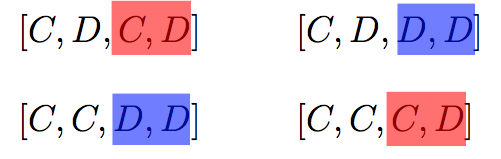
\includegraphics[scale=0.5]{figures/crossover-example.png}
    \caption{Crossover example for genome size 4}
\end{figure}

This cross over is applied to each adjacent pair of prisoners in the current
generation.  Since the order of the prisoners is random, it follows that the pairings
are also random.

\subsection{Mutation}
\label{mutation}

The mutation phase is also easy to follow.  Each gene of the genome is changed
to a random decision $d = Rand \in [C, D]$ with a probability of $p$.  Generally
this value of $p$ is low (between one and five percent) to avoid creating unstable
evolution while still introducing some element of randomness.

\pagebreak
% stupid figure wont fit correctly without this page break (lol)

\subsection{Varying Population Size and Number of Generations}
\label{vpg}
\begin{figure}[h!]
    \centering
    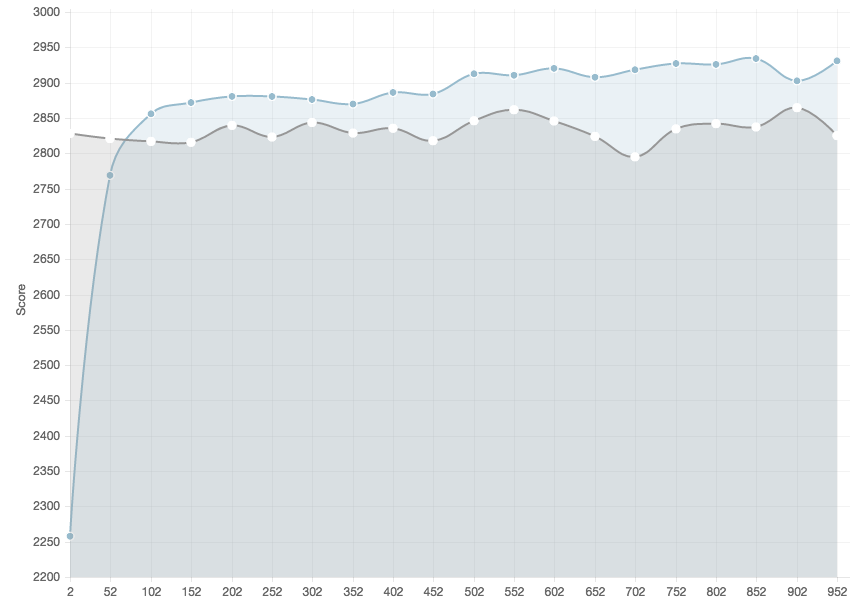
\includegraphics[scale=0.5]{figures/gen_pop_compare}
    \caption{Blue line represents varying population, grey line varying generations}
\end{figure}

While all other factors remain constant,
varying population size has a greater effect on the score when compared to varying the number
of generations in the evolution. As seen in the graph above, increasing the number
of generations has almost no effect on score while increasing the population
size shows a clear upward trend.  It is likely this phenomenon occurs because the genome
strings converge rather quickly.  Increasing population size diversifies
the gene pool and gives a more optimal convergence point. Whereas, increasing
the number of generations simply moves along the asymptote non-productively.

\section{Hill Climbing}

The hill climbing algorithm has a structure equivalent to: \\

\begin{algorithm}[H]
 \KwInput{Initial Prisoner}
 \KwOutput{A prisoner with performance >= the initial prisoner}
 \For{$i\leftarrow 1$ \KwTo $iterations$}{
  $succ$ $\leftarrow$ Mutate($init$)\;
  \If{Fitness($succ$) > Fitness({$init$})}{
   $init$ $\leftarrow$ $succ$\;
  }
 }
 \KwRet{$succ$}
\end{algorithm}

\subsection {Successor Function}

One of the main complications encountered when deriving a successor for any given prisoner
is that there does not exist a natural relationship operator between two prisoners.
As a consequence, successors must be determined using random mutation.  Using
random mutation to compute successors completely nullifies the locality aspect
of the hill climbimg search as it introduces a high probability of moving to an entirely different
section in the search space.  This loss of locality eliminates the usefulness of
methods, such as random restarts and horizontal shoulder movements, which attempt to
escape plateaus and local maxima.

\subsection {Fitness Function}

As \textit{\hyperref[tft]{Score Against TFT}} was previously proved to be the most
effective method for evaluating a prisoner's performance, and the definition
of a strong prisoner is universal across all algorithms, it was re-used as the fitness
function of choice for hill climbing.

\pagebreak

\subsection{Varying Number of Iterations}
\begin{figure}[h]
    \centering
    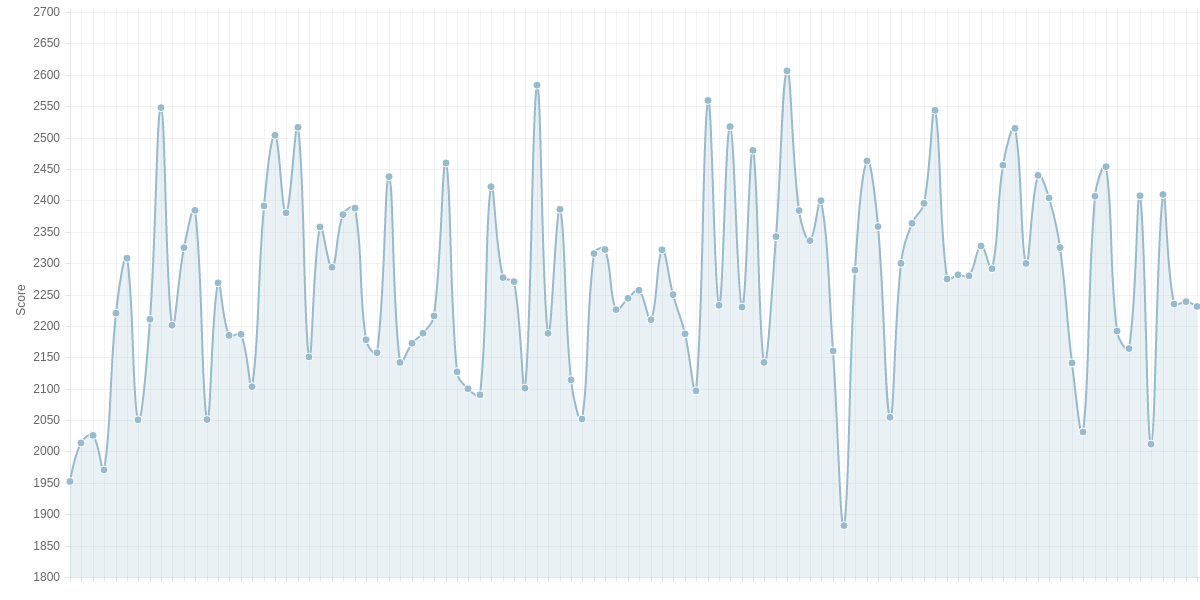
\includegraphics[scale=0.4]{figures/hill_climb.png}
    \caption{Score with respect to iterations between 1 and 1000}
\end{figure}

As seen in the figure above there no is strong correlation between the number
of iterations performed and average score of the prisoner produced.  In fact, the results
are quite sporadic, with major performance decreases occurring throughout.  This is
likely due to the non-local successor function as it implies there is no deterministic way
to improve a solution.

\pagebreak

\section{An Additional Approach}

We simulated the Iterative Prisoners Dilemma problem using a Hill Climbing and Genetic algorithm. But, these two are but a few in a list of possible approaches. Another possible idea is to use a Machine Learning approach, Reinforced Learning. Unlike Supervised Learning, which is given a mapping of states to potential solutions, Reinforced Learning is provided no mapping, making it a more difficult solution. Reinforced Learning is based on the idea that if a favorable result is produced by an action then said action should be "reinforced" or used more often. Although, when an action produces an unfavorable result then the action should be "weakened" or have its use limited. An example of a Reinforced Learning algorithm is Q-Learning. Q-Learning is a model-free learning technique which can be used to acquire a favorable action-selection policy for any given Markov Decision Process. This makes it a suitable approach for Game Theory like problems, for example, the Iterative Prisoners Dilemma problem, where there are repeated simulations against an unknown opponent. Furthermore, Q-Learning can be viewed as a respectable choice because we do not have a clear end goal or overview of the problem environment. Since we compared the results of Hill Climbing to a Genetic algorithm we did not generate resultant data for a Q-Learning approach. Although, passed experiments have shown positive results when compared to a TFT agent. \footnote{\href{http://www.agent.ai/doc/upload/200302/sand95_5.pdf}
{Multiagent Reinforcement Learning in the Iterated Prisoner's Dilemma}}

\pagebreak

\section{Conclusion}

\subsection{Traits of a Strong Genome}
After extensive testing and experimentation, it was discovered that the most successful prisoners
had a bias towards cooperating with their opponent. Most notably, a large portion of
the well performing prisoners choose to cooperate on the first move.
It was observed that rather than immediately responding to the most recent moves, these prisoners would
typically alternate in small bursts between cooperating and defecting. A consistent
pattern between the lengths of these intervals was not immediately obvious, although
the periods of cooperation were generally longer than those of defection.

\subsection{Genetic Algorithm vs Hill Climbing}
The genetic algorithm was able to consistently produce prisoners who performed
optimally against other generated and predefined strategies. This was not the
case however for the prisoners generated by hill climbing. Most prisoners created with this method struggled to outperform their opponents
and were routinely bested in tournament play. \\

The Iterated Prisoner's Dilemma is not a problem well suited for hill climbing.
The lack of a natural successor function for a given strategy makes it impossible
to generate neighouring states which preserve locality.  In addition, since
a solution to the problem does not exist, there is no clear goal for the hill climbing algorithm
to strive for. \\


Prisoners resulting from genetic evolution wholly dominated those resulting
from hill climbing.  The lowest scoring genetic prisoners were able to outscore
the best of the hill climbers.  Genetically evolved prisoners learned the benefits
of mutual cooperation, but also understood the danger of defection.

\pagebreak

\section{Source Code}
All source code for this study was written in C++ and is
available on
\href{https://github.com/Quinny/IteratedPrisoners}{Github}.

\end{document}
